\documentclass{article}
\usepackage[margin=2cm]{geometry}
\usepackage{graphicx}
\usepackage[pages=some]{background}
\usepackage{titling}
\usepackage{tabularx}
\usepackage{tikz}
\usepackage{forest}
\usepackage{float}
\usepackage{color}
\usepackage{tcolorbox}
\usepackage{amssymb}
\usepackage{amsmath}
\usepackage{subfigure}
\usepackage{ragged2e}
\usepackage{multicol}
\usepackage{hyperref}


\forestset{
  my box/.style={
    draw,
    rectangle,
    rounded corners,
    fill=gray!20,
    inner sep=6pt,
    minimum width=3cm % Adjust the width as needed
  }
}


\geometry{a4paper}

\backgroundsetup{
    scale=1,
    angle=0,
    opacity=1,
    contents={%
        
\includegraphics[width=\paperwidth,height=\paperheight]{institution_logo.jpg}
    }
}

\newcommand{\subtitle}[1]{
    \posttitle{
        \par\end{center}
        \begin{center}\large#1\end{center}
        \vskip0.5em}
}

\title{ME-417}
\author{Md. Hasibul Islam}
\subtitle{INTERNAL COMBUSTION ENGINES}

\begin{document}
\begin{titlepage}
    \centering
    
    {\Huge\bfseries\maketitle}
    \textbf{Kazi Arafat Rahman Sir} \\
    \vspace{2cm}
    
\includegraphics[width=8cm]{institution_logo.jpg}
    \vfill
    \vspace*{2cm}
\end{titlepage}

\tableofcontents
\pagebreak
\section{Lecture 01: Introduction to IC Engines} 
\subsection*{\hfill Date: 04/06/2023}

\subsection*{Basics}
IC Engines → CI (Compression ingition), SI (Spark Ignition), Gas Turbine engines \footnote{But this course will cover only CI \& SI engines}\\

\subsubsection*{Key points}
\begin{itemize}
	\item pressure force will give thrust to piston.
	\item combustion will result in expansion.
	\item piston mechanism → mechanical movement.
\end{itemize}

\subsection*{Free Piston Engine}
\subsubsection*{Drag Mechanism}
\subsubsection*{clutch Mechanism} 

\vspace{1cm}

\subsection*{Methods of ignition}
\subsubsection*{Spark Ignition}
spark ignition (SI) is the method used in gasoline engines to ignite the fuel-air mixture using a spark plug.

\subsubsection*{Compression Ignition}
compression ignition (CI) is the process in diesel engines where the fuel ignites due to the high temperature and pressure generated by compressing the air inside the combustion chamber, without the use of a spark plug.


\subsection*{Cycle}
\subsubsection*{2 Stroke}
Combustion process completed in two strokes—compression and ignition, followed by exhaust and intake.

\subsubsection*{4 Stroke}
Combustion process completed in four strokes—intake, compression, power, and exhaust.
\vspace{0.5cm}

\subsection*{Valve}
\subsubsection*{In Head}
Valves positioned in the cylinder head for efficient airflow control.

\subsubsection*{In Block}
Valves integrated into the engine block for simplified construction and maintenance.

\begin{figure}[H]
  \centering
  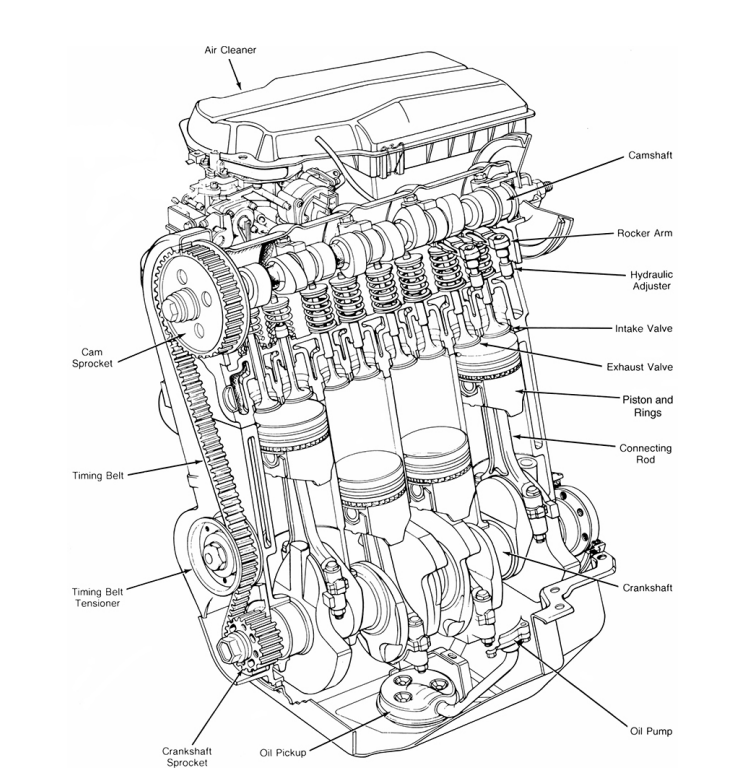
\includegraphics[width=0.75\textwidth]{img/design.png}
  \caption{Basic Design of IC engines.}
  \label{fig:ic engine basic design}
\end{figure}

\subsection*{Types of Cooling}
\subsubsection*{Air Cooling}
Uses air circulation around engine components for heat dissipation.

\subsubsection*{Liquid Cooling}
\begin{itemize}
	\item \textbf{Water Cooling}: Circulates water as a coolant.
	\item \textbf{Liquid-Glycol Cooling}: Mixture of water and glycol to prevent freezing.
\end{itemize}

\subsubsection*{Oil Cooling}
Uses engine oil to absorb heat from components.

\subsection*{Position and number of Cylinders of reciprocating engines}
\subsubsection*{Position of cylinders}
\begin{itemize}
	\item \textbf{Inline}: Cylinders are arranged in a straight line, typically in a row or series.
\item \textbf{V-Type}: Cylinders are arranged in two banks or rows at an angle, forming a "V" shape.
\item \textbf{Flat/Boxer}: Cylinders are horizontally opposed, positioned on opposite sides of the engine and lying flat.
\item \textbf{Radial}: Cylinders are arranged in a circular pattern around a central crankshaft, resembling spokes of a wheel.
\end{itemize}

\subsubsection*{Number of Cylinders}
\begin{itemize}
	\item Single-cylinder: One cylinder in the engine.
	\item Twin-cylinder: Two cylinders.
	\item Inline (e.g., 4-cylinder, 6-cylinder): Multiple cylinders arranged in a straight line.
	\item V-Type (e.g., V6, V8): Multiple cylinders arranged in a "V" configuration.
	\item Flat/Boxer (e.g., 4-cylinder boxer): Multiple horizontally opposed cylinders.
	\item Radial (e.g., 9-cylinder radial): Multiple cylinders arranged in a circular pattern.
\end{itemize}

\begin{figure}[H]
  \centering
  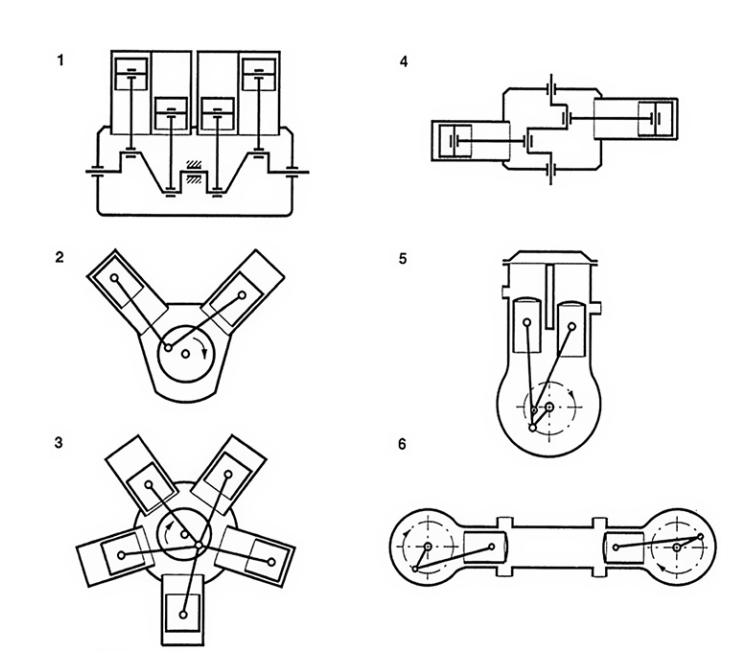
\includegraphics[width=0.65\textwidth]{img/cylinders.png}
  \caption{position \& number of cylinders in reciprocating engines.}
  \label{fig:engine configuration}
\end{figure}

\subsection*{Methods of fuel input for spark ignition engines}
\subsubsection*{Port Fuel Injection (PFI):}
Fuel is injected into the intake ports or manifold before entering the combustion chamber.
\subsubsection*{Direct Fuel Injection (DI):}
Fuel is injected directly into the combustion chamber for precise control and improved efficiency.
\vspace{0.5cm}
\subsection*{Air Intake process}
\begin{itemize}
	\item Air is filtered to remove contaminants.
	\item Throttle valve controls air flow.
	\item Intake manifold distributes air to cylinders.
	\item Air enters combustion chamber for mixing with fuel.
\end{itemize}

\paragraph*{Supercharged}
\begin{itemize}
	\item \textbf{Mechanism}: A supercharger is a mechanical device driven by the engine's crankshaft that forces more air into the combustion chamber. It uses a belt or chain connected to the engine to compress the intake air, resulting in increased air density and more fuel combustion.
	\item \textbf{Advantage}: Supercharging provides instant power boost across the entire RPM range, improving engine performance and responsiveness. It can deliver higher power outputs compared to naturally aspirated engines.
	\item \textbf{Disadvantage}: Supercharging requires engine power to drive the compressor, which results in increased mechanical load on the engine. This can reduce overall engine efficiency and increase fuel consumption.
\end{itemize}

\paragraph*{Turbocharged}
\begin{itemize}
	\item \textbf{Mechanism}: A turbocharger uses the engine's exhaust gases to drive a turbine connected to a compressor. The turbine spins the compressor, compressing the intake air before it enters the combustion chamber. This allows more air and fuel to be burned, resulting in increased power output.
	\item \textbf{Advantage}: Turbocharging improves engine power and efficiency by utilizing wasted exhaust energy. It provides a good balance of power and fuel economy, especially at high RPMs.
	\item \textbf{Disadvantage}: Turbo lag, which is the delay in boost response, can occur due to the time it takes for the exhaust gases to spool up the turbocharger. Additionally, the increased complexity and heat generated by the turbocharger system may require additional cooling measures.
\end{itemize}

\subsection*{Engine components \& Materials}
\subsubsection*{Components of 4 stroke cycle SI engine}
\begin{itemize}
\item \textbf{Cylinder Block}: The main body of the engine that houses the cylinders.

\item \textbf{Cylinder Head}: Covers the top of the cylinder block and contains the combustion chamber, valves, and spark plugs.

\item \textbf{Piston}: Moves up and down within the cylinder, transmitting the force generated by combustion to the connecting rod.

\item \textbf{Connecting Rod}: Connects the piston to the crankshaft, converting the reciprocating motion of the piston into rotary motion.

\item \textbf{Crankshaft}: Converts the linear motion of the pistons and connecting rods into rotary motion, providing power to the drivetrain.

\item \textbf{Intake Valve}: Controls the flow of air-fuel mixture into the combustion chamber during the intake stroke.

\item \textbf{Exhaust Valve}: Controls the flow of exhaust gases out of the combustion chamber during the exhaust stroke.

\item \textbf{Spark Plug}: Provides an electrical spark to ignite the air-fuel mixture in the combustion chamber during the power stroke.

\item \textbf{Intake Manifold}: Distributes the air-fuel mixture to the individual cylinders.

\item \textbf{Exhaust Manifold}: Collects and channels the exhaust gases away from the combustion chamber.

\item \textbf{Camshaft}: Controls the opening and closing of the intake and exhaust valves.

\item \textbf{Timing Belt/Chain}: Synchronizes the rotation of the crankshaft and camshaft to ensure proper valve timing.

\item \textbf{Lubrication System}: Supplies oil to lubricate engine components and reduce friction.

\item \textbf{Cooling System}: Helps regulate engine temperature by circulating coolant to remove excess heat.

\item \textbf{Fuel Injection System}: Delivers the precise amount of fuel to the combustion chamber for efficient combustion.
\end{itemize}

\subsubsection*{Materials of 4 Stroke cycle SI engine}
\begin{itemize}
	\item \textbf{Cylinder Block}: Typically made of cast iron or aluminum alloy.

	\item \textbf{Cylinder Head}: Usually made of aluminum alloy or cast iron.

	\item \textbf{Pistons}: Often made of aluminum alloy with steel reinforcement in critical areas.

	\item \textbf{Connecting Rods}: Commonly made of steel or aluminum alloy.

	\item \textbf{Crankshaft}: Typically made of forged steel for strength and durability.

	\item \textbf{Intake and Exhaust Valves}: Made of materials such as stainless steel, steel alloys, or even titanium alloys for high-performance engines.

	\item \textbf{Valve Springs}: Typically made of steel.

	\item \textbf{Camshaft}: Made of steel or cast iron.

	\item \textbf{Timing Belt/Chain}: Timing belts are usually made of rubber with embedded cords made of materials like fiberglass or kevlar. Timing chains are typically made of steel.

	\item \textbf{Bearings}: Main and connecting rod bearings are often made of steel with a thin layer of bearing material such as aluminum or bronze.

	\item \textbf{Gaskets and Seals}: Made of materials such as rubber, cork, or metal composites to ensure proper sealing.

	\item \textbf{Engine Block Skirt}: Made of cast iron or aluminum alloy.

	\item \textbf{Oil Pan}: Typically made of stamped steel or cast aluminum.

	\item \textbf{Cooling System Components}: Radiator, hoses, and coolant reservoir are commonly made of materials like aluminum, plastic, or rubber.

	\item \textbf{Fuel Injection System Components}: Fuel injectors are usually made of materials such as stainless steel, while fuel rails and fuel pump housings are often made of aluminum alloy or plastic.
\end{itemize}
\vspace{1cm}

\setlength{\fboxsep}{7pt} % Adjust the spacing between the text and the border
\setlength{\fboxrule}{1pt} % Adjust the thickness of the border

\fbox{\begin{minipage}{1\textwidth}
\textcolor{red}{These topics are associated with the book: Heywood (IC Engine Fundamentals, 2018)\\ Chapter: 1.1, 1.2, 1.4, 1.5, 1.7.3}
\end{minipage}}

\newpage
\section{Lecture 2: IC Engine Basics}
\hfill {Date: 11/06/2023}
\subsection*{Poppet Valve}
A poppet valve is a type of valve commonly used in internal combustion engines (IC engines) to control the intake and exhaust of gases into and out of the combustion chamber. It is a crucial component for the proper functioning of the engine.A poppet valve consists of a disk-shaped valve head and a valve stem. The valve head seals against a valve seat to prevent the flow of gases when closed and lifts off the seat to allow the flow of gases when opened. The valve stem connects the valve head to the valve actuation mechanism.In an IC engine, there are usually two types of poppet valves: intake valves and exhaust valves. The intake valves allow the fresh air-fuel mixture to enter the combustion chamber during the intake stroke, while the exhaust valves allow the combustion by-products to exit the chamber during the exhaust stroke.The opening and closing of the poppet valves are controlled by a camshaft, which is driven by the engine's crankshaft. The camshaft has specially shaped lobes that push against the valve stems at precise timings to open and close the valves.The poppet valve design offers advantages such as precise control over the valve timing, efficient sealing when closed, and the ability to handle high-pressure and high-temperature environments. It is widely used in various types of IC engines, including gasoline engines, diesel engines, and many others.


\subsection*{Fuel Injection Port}
Fuel injectors are critical components in modern internal combustion engines that deliver fuel into the combustion chamber with precision. The fuel injector ports, also known as fuel injector nozzles or injector orifices, are the openings through which fuel is sprayed into the intake manifold or directly into the combustion chamber. There are several types of fuel injector ports commonly used in engines:
\begin{itemize}
	\item Single-Point Injectors: Single-point injectors have a single fuel injector port located in the intake manifold. They are typically used in older fuel injection systems and deliver fuel to all the cylinders simultaneously.
	\item Multi-Point Injectors: Multi-point injectors have multiple fuel injector ports, usually one for each cylinder, located in the intake manifold. Each port sprays fuel directly into the respective cylinder's intake port. Multi-point injectors offer better fuel distribution and can deliver fuel more precisely to individual cylinders.
	\item Direct Fuel Injectors: Direct fuel injectors, also known as gasoline direct injection (GDI) or direct injection (DI) injectors, spray fuel directly into the combustion chamber rather than into the intake manifold. This type of injector provides better control over the fuel-air mixture, resulting in improved efficiency and power output.
\end{itemize}

\subsubsection*{Points:}
\checkmark \, The fuel injection timing is different in SI and CI engines. In SI engines, it occurs during the intake stroke, while in CI engines, it occurs near the end of the compression stroke.\\
\subsubsection*{what will happen if SI engine fuel is injected in compression stroke :}
Injecting fuel during the compression stroke in a Spark Ignition (SI) engine would lead to a phenomenon called pre-ignition. Pre-ignition occurs when the fuel-air mixture ignites prematurely before the spark plug fires, which can have several negative consequences:
\begin{itemize}
	\item Knocking: Pre-ignition can cause knocking or pinging, which is an uncontrolled combustion process. Knocking produces a knocking sound and results in increased pressure and temperature in the cylinder, potentially leading to engine damage.
	\item Power Loss: Pre-ignition reduces the power output of the engine since the fuel-air mixture ignites at an incorrect timing. This can result in reduced engine performance and lower efficiency.
	\item Engine Damage: The occurrence of pre-ignition can subject the engine components, such as pistons, valves, and cylinder walls, to higher stresses and temperatures than they are designed to withstand. This can lead to damage or even failure of engine parts over time.
	\item Increased Emissions: Pre-ignition can result in incomplete combustion, leading to increased emissions of pollutants such as unburned hydrocarbons (HC), carbon monoxide (CO), and nitrogen oxides ($NO_x$).
\end{itemize}


\subsubsection*{ICE Vocabulary}
\begin{figure}
    \centering
    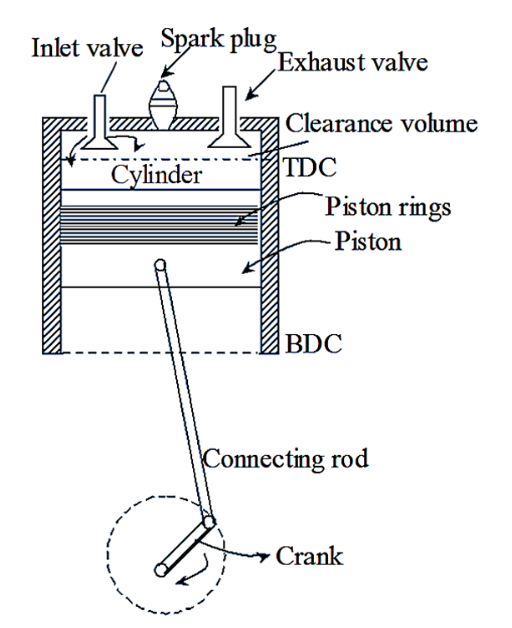
\includegraphics[width=0.5\textwidth]{img/vocabulary.png}
    \caption{ICE terminology}
    \label{fig:ICE terminology}
\end{figure}

\begin{itemize}
	\item \textbf{TDC (Top Dead Center):} It refers to the position of the piston in an engine where it reaches its highest point of travel in the cylinder during the compression or exhaust stroke.

	\item \textbf{BDC (Bottom Dead Center):} It refers to the position of the piston in an engine where it reaches its lowest point of travel in the cylinder during the intake or power stroke.
	
	\item \textbf{Bore:} It refers to the diameter of the cylinder in an engine. It is the measurement of the inner diameter of the cylinder.
	
	\item \textbf{Stroke:} It refers to the distance that the piston travels from TDC to BDC (or vice versa) in the cylinder. It is typically half of the total distance the piston travels in one complete engine cycle.
	\[ \text{Stroke } = \text{TDC} - \text{BDC} \]
	
	
	\item \textbf{Clearance Volume:} It is the volume in the combustion chamber of an engine when the piston is at TDC. It represents the space left at the top of the cylinder when the piston is at its highest point.
	\item \textbf{Swept Volume:} It refers to the total volume of the combustion chamber that is swept or covered by the piston as it moves from its bottom dead center (BDC) position to its top dead center (TDC) position, or vice versa. It is often known as 'cc'.
	\[ \text{swept volume, } V_d = \frac{\pi}{4} \times (\text{bore})^2 \times \text{Stroke} \]

	\item \textbf{Total Volume:} It is the combined volume of the combustion chamber and the clearance volume in an engine. It represents the total capacity of the cylinder when the piston is at BDC. 
		\[ \text{Total volume, } V_t = V_d + V_c \]

		where, $V_c$ is clearance volume \\
		and $V_d$ id swept or displacement volume 

	\item \textbf{Compression Ratio:} It is the ratio of the total volume (including clearance volume) to the clearance volume in the cylinder. It represents the degree of compression of the fuel-air mixture in the cylinder at the end of the compression stroke.
	
	\[ \text{Compression Ratio, } = \frac{V_t}{V_c}\]

	The compression ratio for SI engines usually ranges from 8:1 to 12:1. The compression ratio for CI engines typically ranges from 16:1 to 22:1

\end{itemize}

\subsubsection*{Why CAM profile is made smoother in IC Engine:}
A smoother cam profile in an internal combustion engine is preferred because it reduces wear and friction, improves valve operation, enhances fuel efficiency, reduces noise, and aids in emissions control.

\subsubsection*{What is Blow down:}
Blow down refers to the period when the exhaust valve of an internal combustion engine remains open as the piston moves from the bottom dead center (BDC) to the top dead center (TDC) of the exhaust stroke. This allows the remaining exhaust gases to be expelled from the cylinder before the intake stroke begins.

\subsubsection*{Relation between crackshaft \& camshaft rotation: }
In a four-stroke engine, the crankshaft rotates twice for every single rotation of the camshaft. This is because the four-stroke cycle requires two full rotations of the crankshaft (intake, compression, power, and exhaust strokes) to complete one combustion cycle, while the camshaft completes a full cycle (one revolution) during the same time.


\subsection*{SI Engine Operations}
\begin{itemize}
	\item \textbf{Intake Stroke}: The piston moves from top dead center (TDC) to bottom dead center (BDC), creating a vacuum in the cylinder. The intake valve opens, and the piston moves downward, drawing in a mixture of air and fuel into the cylinder.
	\item \textbf{Compression Stroke}: After the intake valve closes, the piston moves from BDC to TDC, compressing the air-fuel mixture. The compression raises the pressure and temperature in the cylinder, preparing it for combustion.
	\item \textbf{Power Stroke}: At TDC, the spark plug ignites the compressed air-fuel mixture. The rapid combustion produces high-pressure gases that push the piston downward, converting the energy into rotational motion, which is transmitted to the crankshaft.
	\item \textbf{Exhaust Stroke}: As the piston reaches BDC, the exhaust valve opens. The high-pressure gases from the power stroke begin to exit the cylinder, driven by the expanding combustion products. This phase includes the blow down period.
\end{itemize}

\begin{figure}
    \centering
    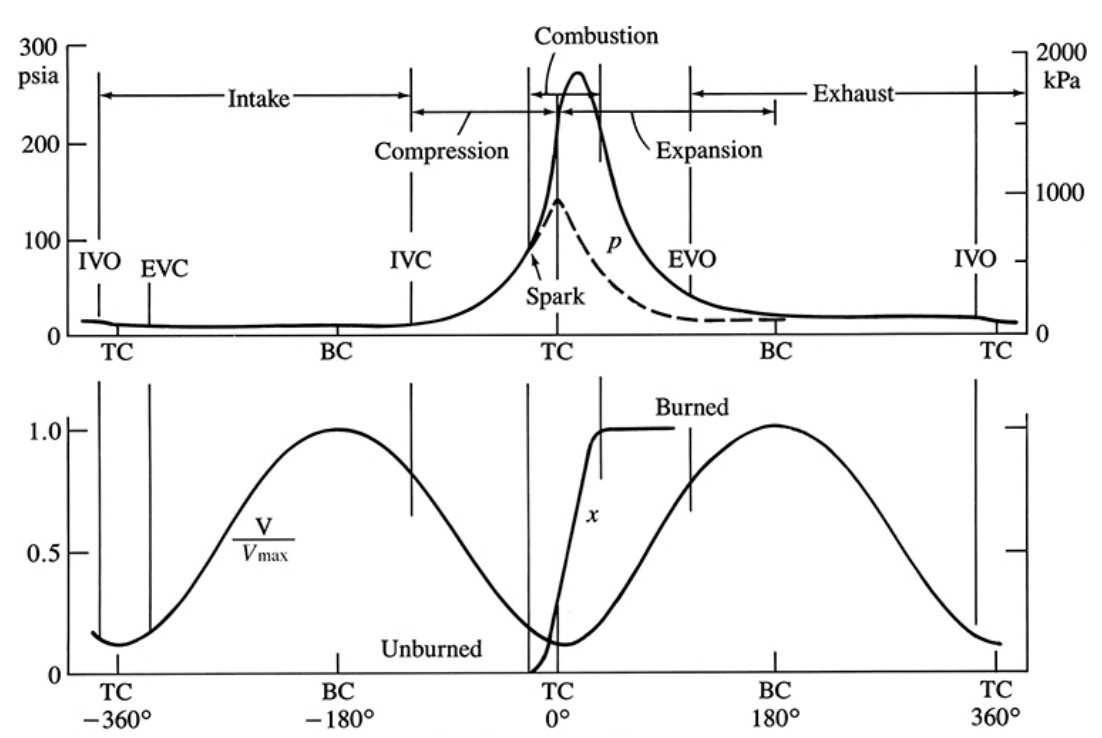
\includegraphics[width=0.8\textwidth]{img/mbt.jpeg}
    \caption{MBT - Maximum Brake Torque Timing}
    \label{fig:mbt_timing}
\end{figure}

\subsubsection*{Some important points:}
\begin{itemize}
	\item \textbf{What is Scavenging:} Scavenging refers to the process of purging or removing the exhaust gases from the combustion chamber of an internal combustion engine. It involves replacing the spent gases with fresh air or air-fuel mixture to improve the combustion process and maximize engine performance. Effective scavenging helps ensure efficient fuel combustion, reduce emissions, and enhance power output.
	\begin{figure}
		\centering
		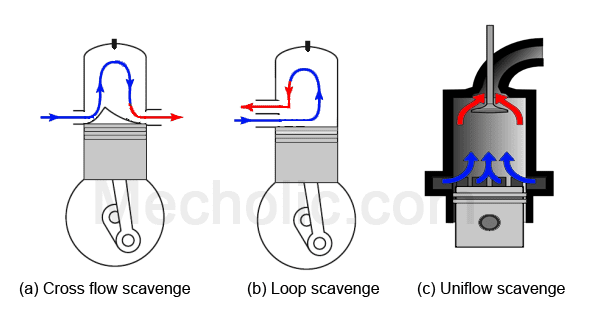
\includegraphics[width=0.8\textwidth]{img/scavenging.png}
		\caption{Types of Scavenging}
		\label{fig:scavenging}
	\end{figure}

	\item \textbf{why IVO (inlet valve open) occurs before EVC (exhaust valve close) in SI engine :} The intake valve opens before the exhaust valve closes in a spark-ignition (SI) engine to promote scavenging of residual gases, enhance cylinder filling, prevent backflow, and optimize engine performance. The period during engine operation when both intake and exhaust valves are open at the same time is called valve overlap. 
	\item \textbf{What will happen if valve overlap is too high:} More fuel is lost through exhaust port. Engine efficiency decreases. Idle stability can be compromised.
	Emissions, especially HC and NOx, increase.
	Low-end torque decreases. Valve train components may experience additional stress and wear.
	
	\item \textbf{How to increase incoming air:} Increasing intake air in a spark-ignition (SI) engine can be achieved through supercharging or turbocharging, both of which compress the intake air to provide more oxygen for combustion, resulting in increased power output.
	\item \textbf{why intake stroke takes longer time than compression stroke:} The intake stroke takes longer than the compression stroke in an internal combustion engine due to factors such as valve opening and closing, airflow resistance, and cylinder filling requirements. The longer duration allows for proper cylinder filling and efficient combustion. Conversely, the compression stroke requires less time as it primarily involves compressing the air-fuel mixture that is already present in the cylinder.

	\item \textbf{Why EVO before completing Expansion stroke:} The exhaust valve opens before the completion of the expansion stroke in an internal combustion engine to facilitate efficient exhaust gas flow, relieve cylinder pressure, promote scavenging, and enable emissions control systems to operate effectively.
	\item \textbf{why IVO pressure is slightly higher than EVC:} The inlet valve opening pressure is set slightly higher than the exhaust valve closing pressure to ensure efficient cylinder filling, prevent backflow of exhaust gases, manage valve train dynamics, and control gas exchange for optimal engine performance.

\end{itemize}

\subsection*{CI engine operations}
\begin{enumerate}
	\item \textbf{Intake Stroke}: The first stroke of the CI engine is the intake stroke. As the piston moves downward, the intake valve opens, allowing a mixture of air and fuel to enter the combustion chamber. The fuel is typically injected directly into the combustion chamber in a high-pressure fuel spray.

	\item \textbf{Compression Stroke}: In the compression stroke, the piston moves back upward, compressing the air-fuel mixture. The compression ratio in a CI engine is relatively high, typically between 15:1 to 22:1, resulting in a highly compressed charge.
	
	\item \textbf{Combustion (Power) Stroke}: As the piston nears the top of the compression stroke, the fuel mixture reaches its autoignition temperature due to the high pressure and temperature within the combustion chamber. This causes the fuel to spontaneously ignite, creating a controlled explosion. The rapid expansion of the ignited gases pushes the piston downward with significant force, generating power.
	
	\item \textbf{Exhaust Stroke}: After the power stroke, the piston starts moving upward again, pushing the burned gases out of the combustion chamber. The exhaust valve opens, and the exhaust gases are expelled through the exhaust manifold and out of the engine through the exhaust system.
\end{enumerate}

\begin{figure}
	\centering
  
	\subfigure[ Cylinder volume/clearance volume V/Vc]{
	  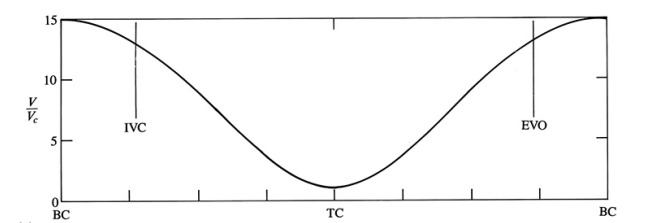
\includegraphics[width=0.45\linewidth]{img/ci_op1.jpeg}
	  \label{fig:image1}
	}
	\hfill
	\subfigure[ rate of	fuel injection $m_{fi}$,]{
	  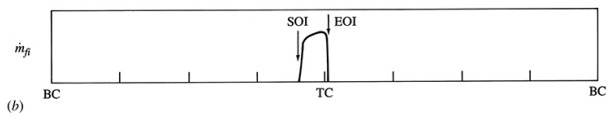
\includegraphics[width=0.45\linewidth]{img/ci_op2.jpeg}
	  \label{fig:image2}
	}
	
	\subfigure[cylinder pressure p (solid line, firing cycle; dashed line, motored cycle),]{
	  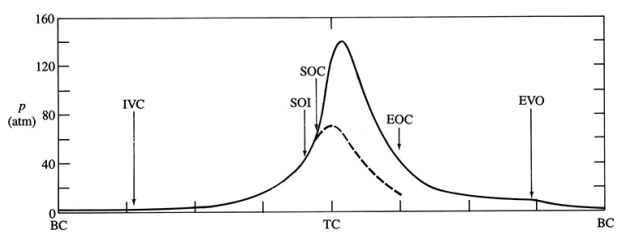
\includegraphics[width=0.45\linewidth]{img/ci_op3.jpeg}
	  \label{fig:image3}
	}
	\hfill
	\subfigure[ rate of fuel burning (or fuel chemical energy release rate) are plotted against crank angle]{
	  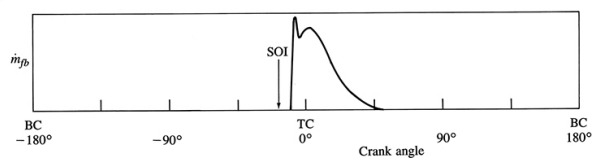
\includegraphics[width=0.45\linewidth]{img/ci_op4.jpeg}
	  \label{fig:image4}
	}
  
	\caption{Sequence of events during compression, combustion, and	expansion processes of a naturally-aspirated compression-ignition engine operating cycle}\footnote[1]{$\checkmark$ SOI = Start of Injection, $\checkmark$ EOI = End of Injection, $\checkmark$ SOC = Start of Combustion}
	\label{fig:overall}
  \end{figure}

 \subsubsection*{Why CI engine is more often than SI engine for two stroke engine:}
 In CI engine, there is no problem if IVO \& EVC time difference is higher. Because, CI engine uses air-fuel mixtures. On the other hand, in SI engine, fuel is used. In that case, more IVO \& EVC time difference may cause a waste of fuel, as fuel come outside while inlet valve is opened. That's why for two stroke engine, CI engine is more used than SI engine. 

 \subsubsection*{Difference between two stroke and Four stroke:}
 \begin{itemize}
	\item \textbf{Simplicity}: Two-stroke engines have a simpler design with fewer moving parts.
	\item \textbf{Power output}: Two-stroke engines tend to have a higher power-to-weight ratio due to their quicker power cycle.
	\item \textbf{Fuel efficiency}: Four-stroke engines are generally more fuel-efficient than two-stroke engines.
	\item \textbf{Emissions}: Two-stroke engines typically produce higher levels of emissions due to the mixture of fuel and lubricating oil.
	\item \textbf{Lubrication}: Two-stroke engines require oil to be mixed with the fuel for proper lubrication, while four-stroke engines have a separate oil system for lubrication.
 \end{itemize}

 \subsubsection*{Types of Scavenging}
 \begin{itemize}
	\item Cross scavenging 
	\item loop scavenging 
	\item uniflow scavenging 
 \end{itemize}

 \section{Lecture 03: IC Engines Cycles} 
\hfill Date: 18/06/2023 \\ 
IC engiine combustion cylinder is an open system, as here mass changes. There's no thermodynamic cycle here, rather it's a operating cycle. Operating cycle consists of multiple operating process. Here, ideal gas model is assumed, hence $C_v,C_p$ are constant. 

\begin{table}[htbp]
	\centering
	\begin{tabularx}{\linewidth}{ p{0.33\linewidth} p{0.66\linewidth}}
	  \hline
	  \multicolumn{1}{c}{Process} & \multicolumn{1}{c}{Assumptions} \\
	  \hline
	  Compression(1-2) & 1. Adiabatic and reversible (hence isentropic) \\
	  \hline
	  Combustion (2-3) & \begin{enumerate}
			\item Adiabatic 
			\item Combustion occurs at: 
				\begin{enumerate}
					\item Constant volume 
					\item Constant Pressure 
					\item Part at constant volume, part at const. pressure 
				\end{enumerate}
			\item Combustion is complete ($\eta_c = 1$)
		\end{enumerate}
	  \\
	  \hline
	  Expansion (3-4) & 1. Adiabatic and reversible (hence isentropic)\\
	  \hline 
		Exhaust (4-5-6) \& intake(6-7-1) & 
			\begin{enumerate}
				\item Adiabatic 
				\item Valve event occurs at top \& bottom dead center 
				\item No change in cylinder volume as pressure differences across open valve drop to zero. 
				\item Inlet and exhause pressure constant 
				\item Velocity affects negligible  
			\end{enumerate}
		\\
		
		\hline 

	\end{tabularx}
  \end{table}

  \begin{figure}
	\centering
  
	\subfigure[ Real Cycle]{
	  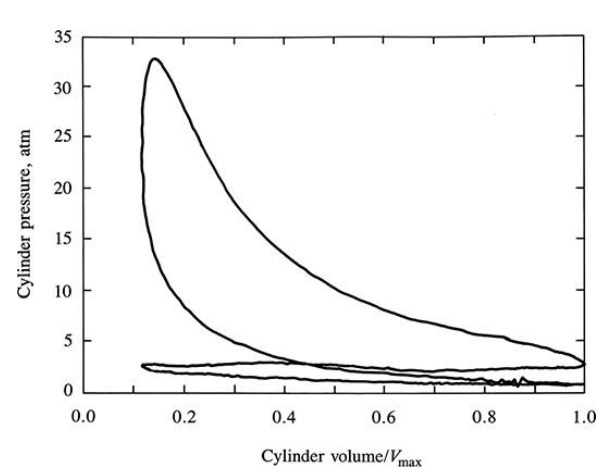
\includegraphics[width=0.45\linewidth]{img/real_cycle.jpeg}
	  \label{fig:real}
	}
	\hfill
	\subfigure[Const volume combustion]{
	  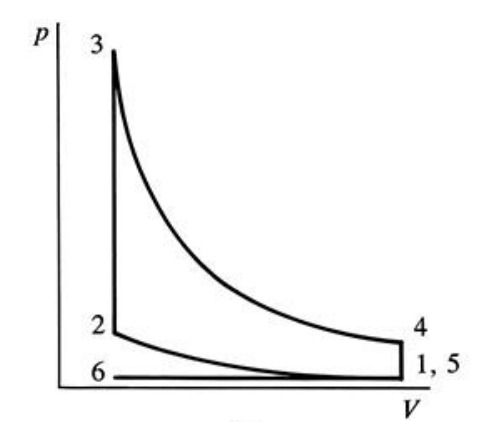
\includegraphics[width=0.45\linewidth]{img/const_vol_cycle.jpeg}
	  \label{fig:const_vol}
	}
	
	\subfigure[Const pressure combustion]{
	  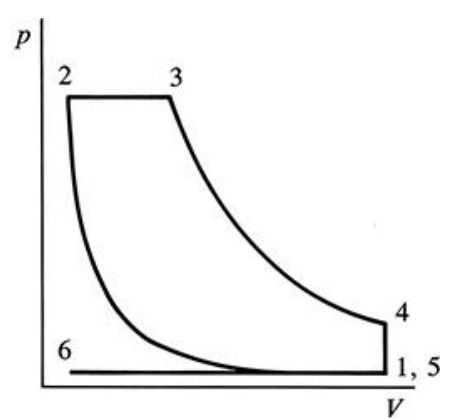
\includegraphics[width=0.45\linewidth]{img/const_pre_cycle.jpeg}
	  \label{fig:const_pressure}
	}
	\hfill
	\subfigure[Limited-pressure combustion]{
	  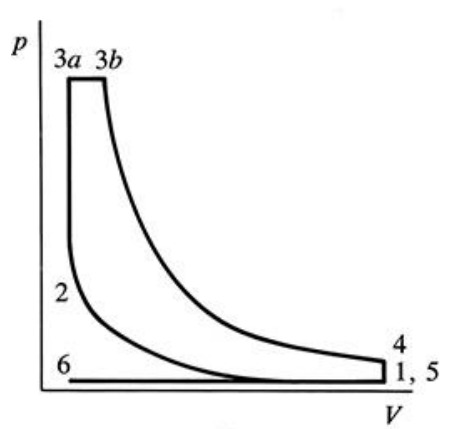
\includegraphics[width=0.45\linewidth]{img/limited_pres_cycle.jpeg}
	  \label{fig:limited_const_vol_pre}
	}
	\subfigure[Throttled constant-volume cycle]{
	  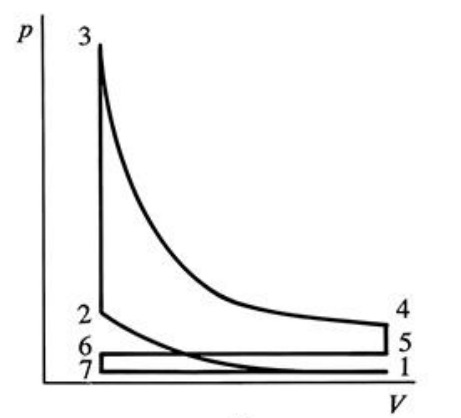
\includegraphics[width=0.45\linewidth]{img/throttle_combustion.jpeg}
	  \label{fig:image5}
	}
	\hfill
	\subfigure[Supercharged constant-volume cycle]{
	  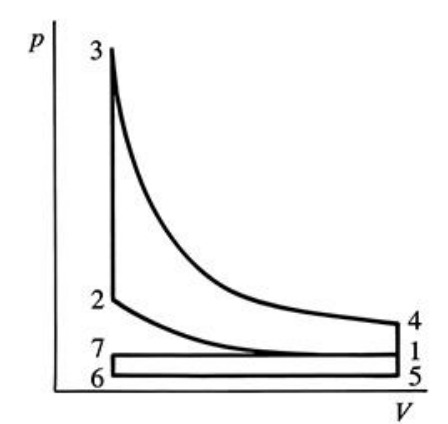
\includegraphics[width=0.45\linewidth]{img/combustion_frg.jpeg}
	  \label{fig:image6}
	}
  
	\caption{Combustion cycle for different case}
	\label{fig:combustion_cycle}
  \end{figure}

  \subsection*{Thermodynamic Relations}
  \begin{multicols}{2}
	\subsubsection*{Nomenclature}
	\begin{itemize}
		\item $W_{C,i}$ = indicated work power
		\item $W_{E}$ = expansion power
		\item $W_{C}$ = compression process power
		\item $\eta_c$ = indicated efficiency 
		\item $m_f$ = mass flow rate of fuel 
		\item $\eta_{t,i}$ = thermal efficiency 
		\item imep = indicated mean effective pressure 
		\item $V_d$ = displacement volume 
		\item $r_c$ = volume ratio 
		\item u = internal energy, U = specific internal energy 
		\item h = enthalpy, U = specific enthalpy 
		\item S = entropy 
		\item LHV = Lower Heating Value
		\item $h = u + pv $
	\end{itemize}
	$$\eta_{f,i} = \frac{W_{c,i}}{m_f Q_{LHV}}$$
	$$\eta_{t,i} = \eta_c \times \eta_{f,i}, \text{,here, } \eta_c=1 $$
	$$imep = \frac{W_{c,i}}{v_d} = \eta_{f,i} \times m_f \times \frac{Q_{LHV}}{V_d}$$
	$$W_{C,i} = W_E + W_C$$
	\subsubsection*{Compression Process}
	$$\frac{v_1}{V_2} = r_c \text{, and } S_1 = S_2$$
	$$W_C = U_1-U_2 = m(u_1-u_2)$$
	
	\subsubsection*{Combustion Process}
	\begin{enumerate}
		\item Const. VOlume : $v_3 = v_2$ and $u_3 - u_2 = 0$
		\item Const. Pressure : $p_e - p_2$ and $h_3 - h_2 = 0$
		\item Limited Pressure Constant: $v_{3a} = v_2$ and $u_{3a}-u_2 = 0$ ; $p_{3b}=p_{3a}$ and $h_{3b} - h_{3a} = 0$
	\end{enumerate}
	\subsubsection*{Expansion Process}
	\begin{enumerate}
		\item Const Volume : $\frac{V_4}{V_3} = r_c$ and $s_4=s_3$\\
		$W_E = U_3 - U_4 = m(u_3-u_4)$
		\item Constant Pressure : $p_3 = p_2, \frac{v_4}{v_2} = r_c \text{ and, } s_4 = s_3$ \\
		\begin{align*}
			W_E &= U_3 - U_4 + p_2(V_3 - V_2) \\
			&= m\left[(u_3-u_4)+ p_2(V_3-V_2)\right] \\
			&= m\left[(u_3 +p_3V_3-u_4-p_4V_4) - p_2V_2 - p_4V_4 \right] \\ 
			&= m\left[(h_3-h_4)+ p_4V_4 - p_2V_2\right]
		\end{align*}
		\item Limited Pressure Const : $\frac{V_4}{V_3a} = r_c$, $p_{3b}=p_{3a}$ and $s_4=s_{3b}$
		$W_E = m\left[(h_{3b}-h_4) + p_4V_4 - p_eV_{3a}\right]$
	\end{enumerate}

	\subsubsection*{Efficiency}
	\begin{enumerate}
		\item Const volume : $$\eta_{f,i} = \frac{m\left[(u_3-u_4)-(u_2-u_1)\right]}{m_fQ_{LHV}}$$
		\item Const Pressure : $$\eta_{f,i} = \frac{m\left[(h_3-h_4)-(u_2-u_1) + p_4V_4 - p_2V_2\right]}{m_fQ_{LHV}}$$
		\item Limited Pressure Const : $$\eta_{f,i} = \frac{m\left[(h_3-h_4)-(u_2-u_1) + p_4V_4 - p_3V_{3a}\right]}{m_fQ_{LHV}}$$
	\end{enumerate}
  \end{multicols}
\vspace*{0.5cm}
  \textbullet Efficiency is very important. There may be residual gases inside and hamper the process.
  \subsubsection*{Blowdown \& Gas displacement}
  \begin{figure}[h]
	\begin{center}
		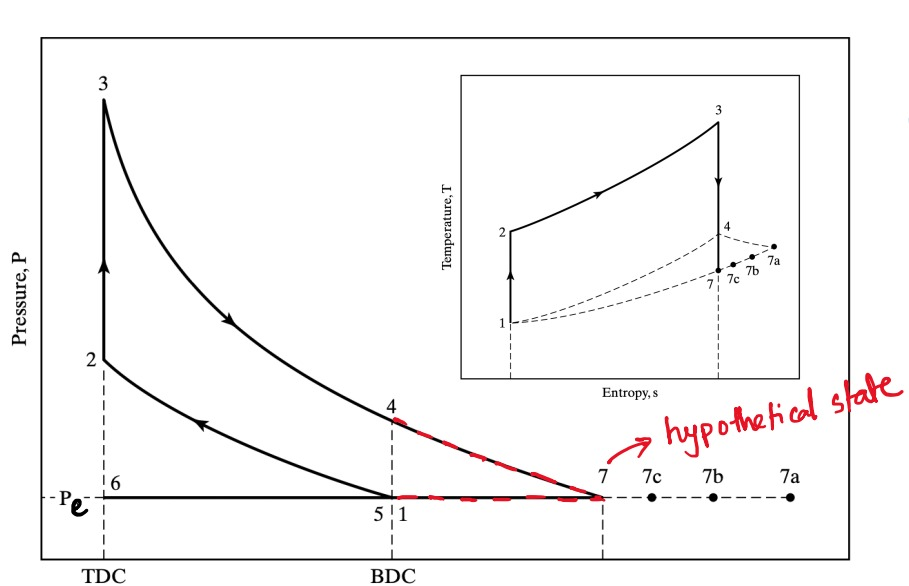
\includegraphics[width=0.75\linewidth]{img/hypothetical_state.jpeg}
		\caption{Hypothetical State}
	\end{center}
  \end{figure}
  At hypothetical point (7), 
  $$p_7 = p_e$$ 
  $$T_7 = T_4 \left(\frac{p_7}{p_4}\right)^\frac{\gamma - 1}{\gamma}$$

  \textbullet The better exhaust, the less residual and better intake will occur. CI engine has less residuals after exhause. \\
  
  \subsubsection*{Blowdown}
  Blowdown in an IC engine refers to the process of expelling burned gases during the exhaust stroke. It involves opening the exhaust valve(s) to release high-pressure exhaust gases, allowing fresh air-fuel mixture to enter the combustion chamber. Blowdown improves gas exchange, relieves pressure, and aids in thermal management of the engine. Timing the opening and closing of the exhaust valve(s) is critical for optimizing engine performance and efficiency.

  \subsubsection*{Exhaust Mechanism}
  \begin{itemize}
	\item The exhaust valve opens to allow the high-pressure exhaust gases to exit the cylinder.

	\item As the exhaust gases are expelled, the pressure inside the cylinder decreases due to the expansion of the gases.
	
	\item The temperature of the exhaust gases also decreases as they expand and lose energy.
	
	\item The first molecule to exit the cylinder has high pressure and kinetic energy. However, as subsequent molecules exit, their kinetic energy decreases as energy is transferred to the surrounding exhaust system.
	
	\item The volume of the combustion chamber expands as the piston moves away from the cylinder head, creating more space for the exhaust gases to occupy.
	
	\item The expansion of the exhaust gases aids in the removal of combustion by-products, including carbon dioxide, water vapor, and unburned hydrocarbons.
	
	\item The decreasing pressure and temperature of the exhaust gases contribute to the thermal management of the engine by reducing the heat buildup within the combustion chamber.
	
	\item Sonic flow, which refers to the flow of gases at the speed of sound, may occur in certain parts of the exhaust system but is typically not present in the cylinder itself during the exhaust stroke.
  \end{itemize}
  \vspace*{1cm}
  \textbf{Reference: John B. Heywood, Internal Combustion Engine Fundamentals, 2nded, 2018\\ Chap: 4.1, 5.1, 5.2, 5.3}

  \pagebreak
  \section{Lecture 04: NASA-CEA analysis} 
	\hfill Date: 04/06/2023

	\subsubsection*{NASA CEA Analysis Tools}
	\begin{itemize}
		\item Website: \href{https://cearun.grc.nasa.gov/}{https://cearun.grc.nasa.gov/} 
		\item Python Extension : PyCea 
		\item Matlab Extension also available 
	\end{itemize}
	\textbf{There will a CT regarding reading properties from NASA-CEA }

	\vspace*{1cm}
	\section{Lecture 05: Ideal Gas Constant-Volume cycle anlysis} 
	\hfill Date: 18/07/2023

	\begin{multicols}{2}
		\subsection*{Residual Gas Mass Fraction, $X_r$}
		

		\begin{align*}
			x_r &= \frac{m_{r}}{m} \\
			\Rightarrow m_r &= \frac{V_6}{v_7} = \frac{V_2}{v_7} \\
			&\\
			\text{and } m &= \frac{V_i}{v_i} \, \text{ ; i= 1,2,3,4,7}\\
			&\\
			x_r &= \left(\frac{\frac{V_6}{v_7}}{\frac{V_4}{v_4}}\right) \\
			&= \left(\frac{V_6}{V_4}\right) \left(\frac{v_4}{v_7}\right) \\
			&= \frac{1}{r_c} \times \frac{\frac{RT_4}{P_4}}{\frac{RT_7}{P_7}} \\
			&= \frac{1}{r_c} \times \frac{P_{ex}}{P_4} \times \frac{T_4}{T_7} \\
			&= \frac{1}{r_c} \times \frac{P_{ex}}{P_4} \times \left(\frac{P_4}{P_7}\right)^{\frac{\gamma -1}{\gamma}} \, \text{ [isentropic relation]} \\
			&= \frac{1}{r_c} \left(\frac{P_4}{P_{ex}}\right)^{-1/r} \\
			&= \frac{1}{r_c} \left(\frac{P_{ex}}{P_4}\right)^{1/r} \\
			&= \frac{1}{r_c} \left(\frac{P_{ex}}{P_i} \times \frac{P_1}{P_4}\right)^{1/r}\, [P_{inlet} = P_4] \\
			&\\
			\text{Now, } \frac{P_{1}}{P_4} &= \frac{P_1}{P_2} \times \frac{P_2}{P_3} \times \frac{P_3}{P_4} \\
			&= \left(\frac{V_2}{V_1}\right)^\gamma \frac{T_2}{T_3} \left(\frac{V_4}{V_3}\right)^\gamma \\
			r_c &= \frac{V_1}{V_2} = \frac{V_4}{V_3} \\
			\text{so, } \frac{P_1}{p_4} &= \frac{T_2}{T_3} \\
			&\\
			x_r &= \frac{1}{r_c} \left(\frac{P_{ex}}{P_i}\right)^{1/\gamma} \times \left(\frac{T_2}{T_3}\right)^{1/r} \\ 
		\end{align*}

		\begin{figure}[H]
			\begin{center}
				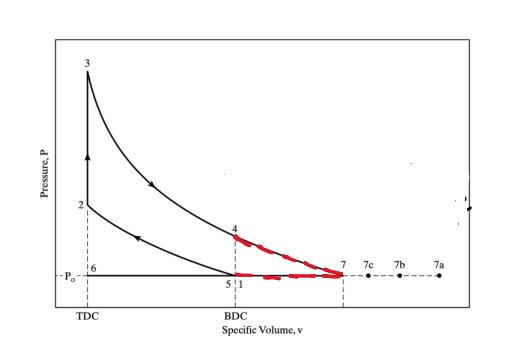
\includegraphics[width=\columnwidth]{img/const_vol_adia_comb_process.jpeg}
			\end{center}
		\end{figure}

		\begin{itemize}
			\item $c_p, c_v$ are constant for ideal gas.
			\item point-7 is a hypothetical point. 
		\end{itemize}

		At constant volume adiabatic combustion process,
		\begin{align*}
			mC_v(T_3-T_2) &= m_f Q_{LHV} \\
			&\\
			\text{Again, }\frac{m_f Q_{LHV}}{m} &= Q^* \\
			&\\
			\text{So, } C_v (T_3-T_2) &= Q^* \\
			\frac{T_3}{T_2} &= 1 + \frac{Q^*}{C_vT_2}
		\end{align*}
		\begin{center}
			\fbox{
			  \begin{minipage}{\columnwidth}
				$$\frac{T_2}{T_1} = \left(\frac{V_1}{V_2}\right)^{\gamma -1} = \left(\frac{V_4}{V_3}\right)^{\gamma -1} = r_c^{\gamma -1} = \frac{T_3}{T_4} $$\\
				$$\therefore \frac{T_4}{T_1} = \frac{T_3}{T_2}$$
			  \end{minipage}
			}
		  \end{center}

		  \begin{align*}
			\text{So, } \frac{T_3}{T_2} &= 1 + \frac{Q^*}{C_v \frac{T_3}{T_4} T_1} \\
			&= 1 + \frac{Q^*}{C_v T_1 r_c^{\gamma -1}} \\
		  \end{align*}

		  \begin{center}
			\fbox{
			  \begin{minipage}{\columnwidth}
				$$x_r = \frac{1}{r_c} \frac{\left(\frac{P_{ex}}{P_i}\right)^{1/\gamma}}{\left[1 + Q^* / \left(C_v T_1 r_c^{\gamma -1}\right)\right]^{1/\gamma}}$$
				\\
				$$x_r\, \, \uparrow \,, \,\, \underbrace{P_i<P_{ex}} \,,\,\, r_c \,\, \downarrow \,,\,\, \frac{Q^*}{C_v T_1} \, \downarrow $$
				\hspace*{2.7cm} \textbf{throttled} \\ 
				\begin{itemize}
					\item $\frac{Q^*}{C_v T_1}$ is dimensionless parameter. Here, $C_v$ changes with temperature. That's why, this whole dimensionless parameter depends upon exhaust temperature. Hence, $x_r$ will also change with temperature.
				\end{itemize}
			  \end{minipage}
			}
		  \end{center}

		  \begin{align*}
			\eta_{f,i} &= \frac{m\left[(u_3-u_4)-(u_2-u_1)\right]}{m_fQ_{LHV}} \\
			&= \frac{\left(T_3-T_4\right) - \left(T_2-T_1\right)}{T_3 - T_2} \\
			&= 1 - \frac{T_4-T_1}{T_3-T_2} \\
			&= 1 - \frac{1}{r_c^{\gamma -1}} \\
			&\\
			& \eta_{f,i} \,\, \uparrow \,\, , \,\, r_c \,\, \uparrow ,\,\, \gamma \, \uparrow 
		  \end{align*}

		  $\gamma$ is change:-
		  \begin{itemize}
			\item If temperature is changed 
			\item If air-fuel mixture burnt, the mixing combination also changed. Hence $\gamma$ is changed. 
		  \end{itemize}

		  \textbf{IMEP (mean effective pressure):} How well displaement volume works.

		  \begin{align*}
			\frac{imep}{P_1} &= \frac{m_f \times Q_{LHV} \times \eta_{f,i}}{V_d P_1} \\
			&= \underbrace{\left(\frac{Q^*}{C_v T_1}\right)} \frac{m T_1 C_v}{V_d P_1} \underbrace{\left(1 - \frac{1}{r_c^{\gamma -1}}\right)} \\
			& \text{dimensionless} \hspace*{1cm} \text{dimensionless}
		  \end{align*}

		  now, 
		  \begin{align*}
			\frac{C_v T_1 V_1/v_1}{(V_1-V_6) P_1} &= \frac{C_v T_1 V_1}{(V_1-V_6) R T_1} \\
			&= \left(\frac{C_v}{C_p - C_v}\right) \left(\frac{1}{1-\frac{1}{r_c}}\right)\\
			&= \left(\frac{1}{\gamma -1}\right) \left(\frac{r_c}{r_c-1}\right)
			&\\
			\therefore \frac{imep}{P_1} &= \left(\frac{Q^*}{C_v T_1}\right) \left(\frac{1}{\gamma -1}\right) \left(\frac{r_c}{r_c-1}\right) \left(1 - \frac{1}{r_c^{\gamma-1}}\right)\\
			&\\
			\text{using, } \frac{T_3}{T_2} &= 1 + \frac{Q^*}{C_v T_1 r_c^{\gamma -1}}
		  \end{align*}

		  We get,
		  $$\frac{imep}{P_3} = \frac{1}{\left(\gamma -1\right) r_c^\gamma} \left(\frac{r_c}{r_c-1}\right) \frac{1 - \frac{1}{r_c^{\gamma-1}}}{\frac{C_v T_1}{Q^*} + \frac{1}{r_c^{\gamma-1}}}$$

		  \begin{itemize}
			\item A higher value of $imep$ is desirable 
			\item $P_3$ should be less, so less stress. $P_3$ is the highest pressure. So, lesser value of $P_3$ is desirable. 
		  \end{itemize}

		  
		\begin{figure}[H]
			\begin{center}
				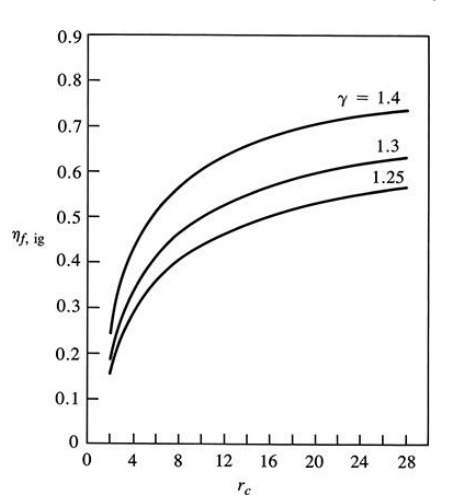
\includegraphics[width=\columnwidth]{img/eff_vs_rc_with_gamma.jpeg}
			\end{center}
		\end{figure}
	\end{multicols}
	\pagebreak
	\subsection*{Cycle Comparison}
	\begin{figure}[H]
		\begin{center}
			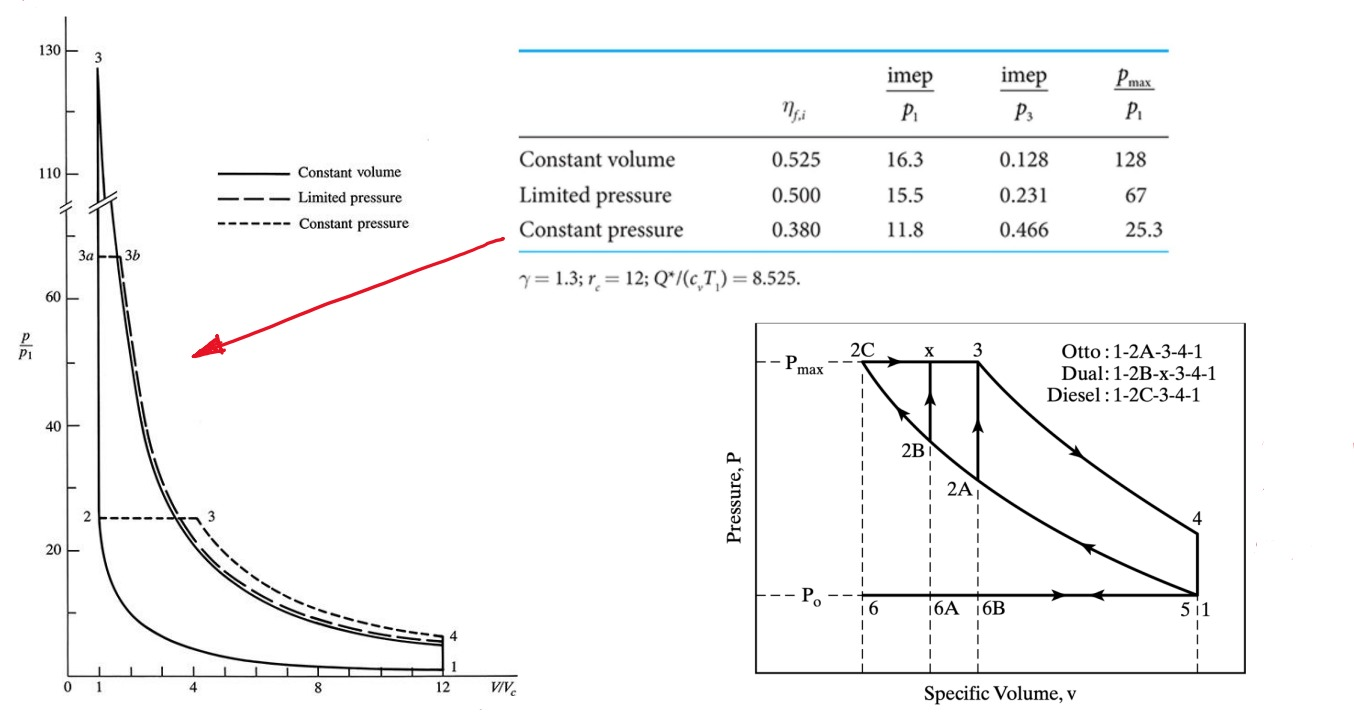
\includegraphics[width=\linewidth]{img/cycle_comparison.jpeg}
		\end{center}
	\end{figure}
	\begin{multicols}{2}
		const volume : $\eta \,\, \uparrow \,$ but, $\frac{imep}{P_3} \,\, \downarrow $\\
		const pressure : $\eta \,\, \downarrow \,$ but, $\frac{imep}{P_3} \,\, \uparrow $\\

		\textbf{Then, efficiency of CI engine is less than SI engine?}\\
		No, Because in CI engine, compression ratio ($r_c$) is higher. As a result, graphically they are more extended to the right side (in Fig. point 4). That's why, The efficiency of CI engine in high although having constant pressure. 

		\begin{itemize}
			\item Graph explaination is important for term final 
		\end{itemize}

		\subsection*{Fuel-Air Ratios}
		\begin{itemize}
			\item $\phi\, \rightarrow$ Equivalence ratio  
			\item $\phi=1$ indicates stoichiometric mixture 
			\item $\phi < 1$ indicates lean mixture 
			\item $\phi > 1$ indicates rich mixture 
			\item Combustion temperature would be highest when $\phi$ is slightly higher than 1. 
			\item $\phi$ can be changed with temperature and air density. 
			\item Equivalence ratio ($\phi$) is behaving like $\gamma$ is air fuel mixing 
			\item With the change of $\phi$, temperature changes, $C_p\, \, \&\,\, C_v$ changes, as a result $\eta$ also changes.  
		\end{itemize}

		\begin{itemize}
			\item Lean mixture $\rightarrow$ higher $\eta$
			\item Rich mixture $\rightarrow$ lower $\eta$
			\item In rich mixture, due to incomplete combustion, efficiency drops. This effect is more than temperature rise, $C_p, C_v$ rise. That's why lean mixture has more efficiency than rich mixtures.
			\item with the change of $\phi$, mixing composition changes, mass fraction changes, also $imep/P_3$ changes.   
		\end{itemize}
	\end{multicols}
	\begin{center}
		\fbox{\hspace*{0.33\linewidth} \textbf{Follow Heywood: 5.3, 5.4, 5.5} \hspace*{0.33\linewidth}} 
	\end{center}
	\pagebreak 

	\section{Lecture 06: Fuel-Air Otto Cycle} 
	\hfill Date: 23/07/2023

	\begin{multicols}{2}
		\begin{itemize}
			\item $imep$ is maximized when $\phi$ is closed to 1. 
			\item Fuel efficiency is better at lean mixture.
			\item \textbf{Inlet pressure or outlet pressure, which one is higher?} Can be equal or different, anything.
			\item $\frac{P_i}{P_e} < 1 \rightarrow$ throttle 
			\item $\frac{P_i}{P_e} > 1 \rightarrow$ supercharged, Turbocharged 
			\item Limited pressure cycle indicates diesel cycle. 
			\item In otto cycle, for lower value of $\phi$ efficiency is higher, which is consistant with limited pressure cycle. 
		\end{itemize}
	\end{multicols}
	\begin{figure}[H]
		\begin{center}
			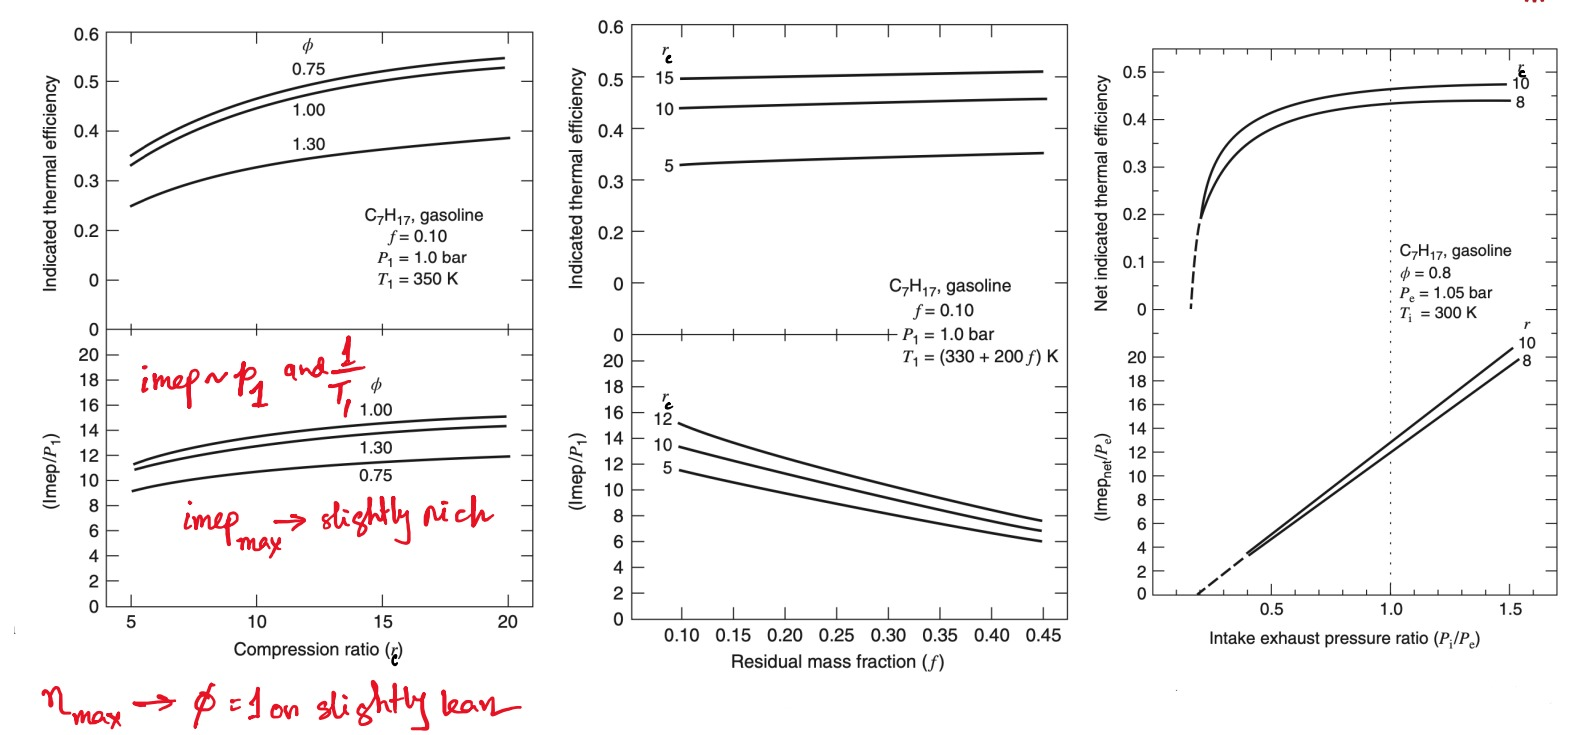
\includegraphics[width=\linewidth]{img/otto_cycle.jpeg}
		\end{center}
	\end{figure}
	\begin{itemize}
		\item Superchargers and turbochargers increase air intake density, allowing more fuel to be burned, boosting power output. However, they do not significantly alter the underlying thermodynamic efficiency, leading to consistent net indicated thermal efficiency.
	\end{itemize}

	\subsubsection*{Overexpanded IC engine}
	\begin{multicols}{2}
		\begin{figure}[H]
			\begin{center}
				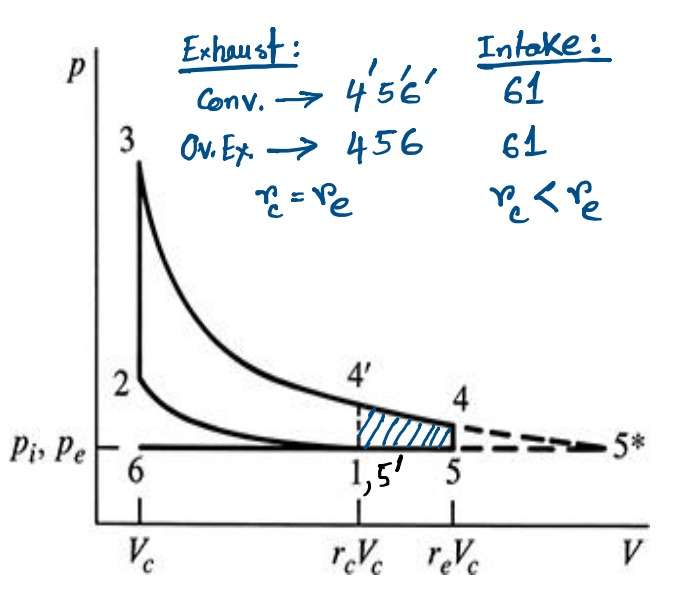
\includegraphics[width=\linewidth]{img/overexpanded.jpeg}
			\end{center}
		\end{figure}
		\begin{itemize}
			\item 6-1: intake 
			\item 1-2: compression 
			\item 2-3: combustion
			\item 3-4': expansion 
			\item 4'-5': blowdown 
			\item 5'-6': exhaust
			\item if we don't blow down in 4'-5', rather expand it more and pass through 4-5, then it's called overexpanded.
			\item $r_c$ = compression ratio, $r_e$ = expansion ratio
			\item conventional: $r_c = r_e$
			\item overexpanded: $r_c < r_e$
		\end{itemize}
		By overexpansion,
		$$r=\frac{r_e}{r_c} \, \, \uparrow, \, \eta_{f,i} \,\, \uparrow \, ,\text{but } \frac{imep}{P_1} \,\,\downarrow$$
		So, we need to turbocharge or supercharge, in order to increase $imep$. 

		\textbf{Physical Interpretation of IMEP}: IMEP (induced mean effective pressure) represents the hypothetical constant pressure that, if exerted on the piston throughout the entire power stroke, would produce the same amount of net work output as the actual varying pressure that occurs during the combustion process.

		\subsubsection*{Real Cycle}
		Losses in real cycle:
		\begin{enumerate}
			\item Heat transfer : through combustion, expansion stroke (2-3, 3-4')
			\item Finite combustion time: If there is no heat transfer, peak pressure would have high. But with overall effect, it's become low. 
			\item Exhaust blowdown loss
			\item Crevice leakage 
			\item Incomplete combustion: Lean or rich, always there would be some incomplete combustion.
			\item combustion occuring less than $P_max$ : limited pressure cycle.
		\end{enumerate}

		\begin{figure}[H]
			\begin{center}
				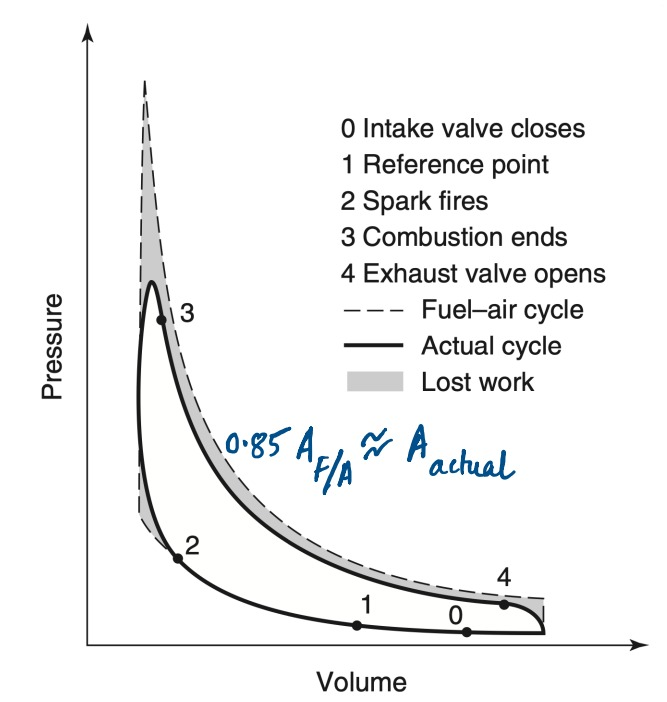
\includegraphics[width=\linewidth]{img/real_cycle_loss.jpeg}
			\end{center}
		\end{figure}
	\end{multicols}
	\begin{center}
		\fbox{\hspace*{0.33\linewidth} \textbf{Follow Heywood: 5.6, 5.8} \hspace*{0.33\linewidth}} 
	\end{center}
	\vspace*{2cm}

	\section{Lecture 07: Exhaust Emission} 
	\hfill Date: 06/08/2023

	\begin{center}
		\fbox{\hspace*{0.33\linewidth} \textbf{Follow Heywood: 11.1, 11.2} \hspace*{0.33\linewidth}} 
		\fbox{\hspace*{0.315\linewidth} \textbf{Follow Colin Ferguson: 8.1, 8.2} \hspace*{0.31\linewidth}} 
	\end{center}

	\section{Lecture 08: Missed the class} 
	\hfill Date: 13/08/2023

	\section{Lecture 09: Formation of Soot} 
	\hfill Date: 20/08/2023
	
	\begin{itemize}
		\item CI engine: CO formation is higher! (why?)
		\item SI engine $\rightarrow$ uniform  
		\item CO formation will be higher at first, then it will decrease after time.
		\item Soot formation: $$C_aH_b + cO_2 \rightarrow 2cCO + b/2 H_2 + (a - 2c) C$$
		\item Turbulence : better mixing \& Less soot 
	\end{itemize}

	\begin{center}
		\fbox{\hspace*{0.28\linewidth} \textbf{Follow Colin Ferguson: 8.3, 8.4, 8.5, 8.6} \hspace*{0.28\linewidth}} 
	\end{center}

\end{document}
